\chapter{Modelo de procesos de negocio}
El modelo de procesos de negocio es una notación gráfica que describe la lógica de los pasos de un proceso de negocio. Esta notación ha sido especialmente diseñada para coordinar la secuencia de los procesos y los mensajes que fluyen entre los participantes de las diferentes actividades.\\

Los diagramas de procesos de negocio son diagramas diseñados para representar gráficamente la secuencia de todas las actividades que ocurren durante un proceso, basado en la técnica de ``Flow Chart", incluye además toda la información que se considera necesaria para el análisis.\\

La diferencia principal entre el modelado de sistemas en UML y Modelado de procesos de negocio es que se hace más énfasis en como se realiza el trabajo en un organización, en lugar de que trabajo se hace.
%--------------------------------------------------------------------------------------------------------
\section{Modelo actual}
Los siguientes diagramas describen los procesos tradicionales y genéricos que se siguen en un centro educativo para la formación de Karate Do.\\

Documentar ésta información es importante porque es la base del análisis y diseño de nuestro trabajo terminal.\\

\begin{enumerate}
	\item \textbf{Inscripción}\\
	Para realizar el entrenamiento de Karate Do, el Practicante tiene que estar inscrito en una clase. La Figura \ref{fig:PN_Actual_Inscripcion} \nameref{fig:PN_Actual_Inscripcion} muestra el procedimiento a seguir para realizar la inscripción donde el Practicante es quien debe solicitar la inscripción personalmente con el Entrenador y éste a su vez registrar los datos personales del Practicante en una ficha de inscripción.\\
	
	\begin{figure}[H]
		\begin{center}
			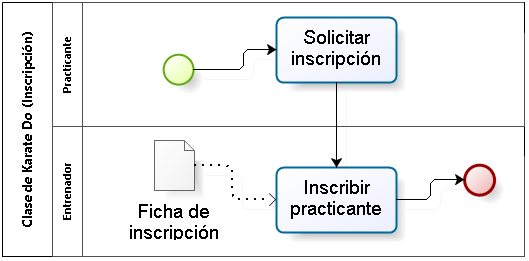
\includegraphics[scale=0.7]{./Figuras/Negocio/Proceso_de_Negocio_actual_inscripcion}
		\end{center}
		\caption{Proceso de negocio actual - Inscripción}
		\label{fig:PN_Actual_Inscripcion}
		%\captionsetup{font={footnotesize,it}}
		%\caption*{Elaboración propia}
	\end{figure}

	\item \textbf{Clase de Karate Do}\\
	Una clase de Karate Do actual consta de 3 partes, el calentamiento, la resistencia y la técnica. La Figura \ref{fig:PN_Actual} \nameref{fig:PN_Actual} muestra el proceso de como se desarrolla una clase de Karate Do.  Para cada una de las partes el Entrenador es quien ejemplifica el ejercicio o movimiento a realizar, después de haber hecho esto, los practicantes replican dicho movimiento y seguido de ello comienzan a realizar repeticiones del mismo. El número de repeticiones del movimiento dependen de lo que el Entrenador establezca. Existen observaciones del Entrenador hacia el Practicante pero no es una tarea que se sigue estrictamente, depende de cada uno de los practicantes y de su desempeño.
	
	\begin{figure}[H]
		\begin{center}
			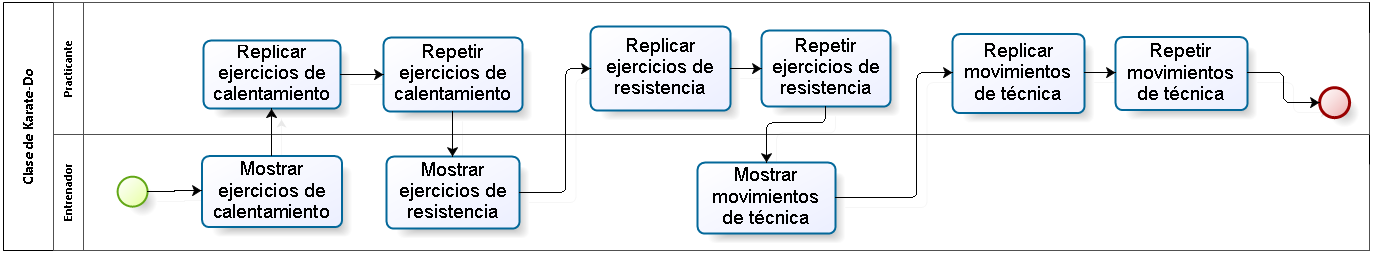
\includegraphics[scale=0.45]{./Figuras/Negocio/Proceso_de_Negocio_actual}
		\end{center}
		\caption{Proceso de negocio actual}
		\label{fig:PN_Actual}
	\end{figure}

\end{enumerate}

%--------------------------------------------------------------------------------------------------------
\section{Modelo propuesto}
El modelo propuesto toma como base el proceso de una clase actual de Karate Do, de donde se toman los ejercicios de calentamiento y los movimientos de técnica delimitados en el \nameref{sec:Alcance} para así desarrollar una herramienta que permita la captura de ejercicios y movimientos para almacenarlos en diferentes rutinas por parte del Entrenador y su posterior replicación por parte de los Practicantes. La Figura \ref{fig:PN_Propuesto} \nameref{fig:PN_Propuesto} muestra la secuencia de acciones que se presenta en el modelo propuesto mediante éste trabajo terminal.\\

\begin{figure}[H]
	\begin{center}
		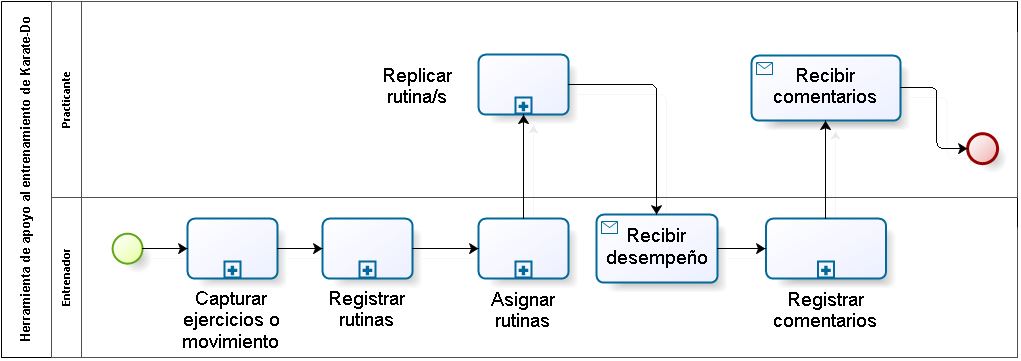
\includegraphics[scale=0.65]{./Figuras/Negocio/Proceso_de_Negocio_propuesto}
	\end{center}
	\caption{Proceso de negocio propuesto}
	\label{fig:PN_Propuesto}
\end{figure}

\begin{enumerate}
	\item \textbf{Registro en la herramienta}\\
	Para poder hacer uso de la herramienta, el Practicante tiene que estar registrado en la misma, para realizar este registro el Practicante lo solicita personalmente al Entrenador y éste escribe los datos personales del Practicante en un formulario de registro de la herramienta tal como lo muestra la Figura \ref{fig:PN_Propuesto_Registro} \nameref{fig:PN_Propuesto_Registro}.\\
	
	\begin{figure}[H]
		\begin{center}
			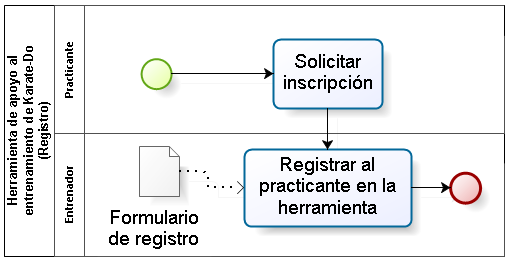
\includegraphics[scale=0.7]{./Figuras/Negocio/Proceso_de_Negocio_propuesto_registro}
		\end{center}
		\caption{Proceso de negocio propuesto - Registro}
		\label{fig:PN_Propuesto_Registro}
	\end{figure}

	\item \textbf{Herramienta de apoyo al entrenamiento de Karate Do}\\
	Para realizar una rutina de entrenamiento a distancia se propone una serie de pasos a realizar dentro de la herramienta los cuales se enlistan a continuación:
	\begin{itemize}
		\item Capturar movimientos (Entrenador): La Figura \ref{fig:procesonegocioP_captEjer} \nameref{fig:procesonegocioP_captEjer} muestra el primer paso para utilizar la herramienta el cual consiste en que el Entrenador capture y guarde los movimientos que utiliza en las rutinas de entrenamiento.
			%Capturar_ejercicios_o_movimientos
			\begin{figure}[H]
				\begin{center}
					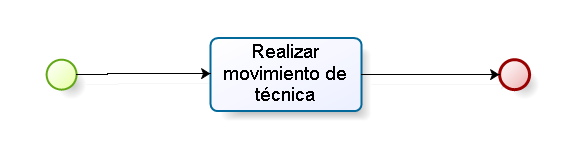
\includegraphics[scale=0.7]{./Figuras/Negocio/Capturar_ejercicios_o_movimientos}
				\end{center}
				\caption{Capturar movimientos}
				\label{fig:procesonegocioP_captEjer}
			\end{figure}
		\item Registrar rutinas (Entrenador): En la Figura \ref{fig:procesonegocioP_regRutinas} \nameref{fig:procesonegocioP_regRutinas} se puede observar que el Entrenador crea las rutinas de acuerdo a su criterio eligiendo de entre los ejercicios de calentamiento y movimientos de técnica que ha capturado previamente.
			%Registrar_rutinas
			\begin{figure}[H]
				\begin{center}
					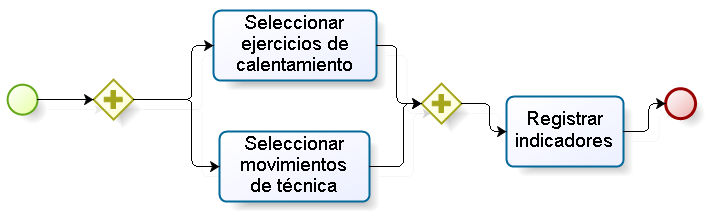
\includegraphics[scale=0.7]{./Figuras/Negocio/Registrar_rutinas}
				\end{center}
				\caption{Registrar rutinas}
				\label{fig:procesonegocioP_regRutinas}
			\end{figure}
		\item Asignar rutinas (Entrenador): Al tener las rutinas registradas, el Entrenador asigna las diferentes rutinas a sus diferentes Practicantes, eligiendo de manera personal las más adecuadas para cada uno de ellos tal como lo muestra la Figura \ref{fig:procesonegocioP_asigRutinas} \nameref{fig:procesonegocioP_asigRutinas}.
			%Asignar Rutinas
			\begin{figure}[H]
				\begin{center}
					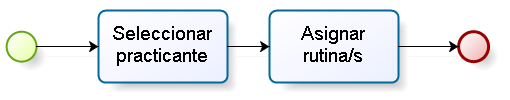
\includegraphics[scale=0.7]{./Figuras/Negocio/Asignar_rutina}
				\end{center}
				\caption{Asignar rutinas}
				\label{fig:procesonegocioP_asigRutinas}
			\end{figure}
		\item Replicar rutinas (Practicante): La Figura \ref{fig:procesonegocioP_repRutinas} \nameref{fig:procesonegocioP_repRutinas} muestra que el trabajo principal del Practicante es la realización de rutinas, es decir replicar los movimientos que el Entrenador le asignó, observando un desempeño final de la rutina el cual además será enviado al Entrenador.
			%Replicar Rutinas
			\begin{figure}[H]
				\begin{center}
					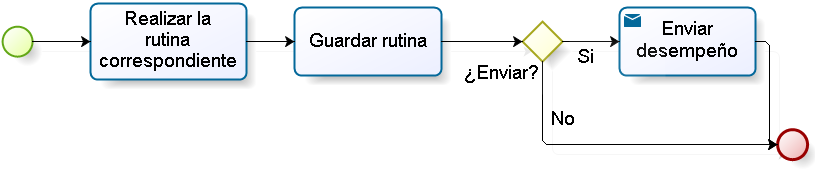
\includegraphics[scale=0.7]{./Figuras/Negocio/Replicar_rutinas}
				\end{center}
				\caption{Replicar rutinas}
				\label{fig:procesonegocioP_repRutinas}
			\end{figure}
		\item Recibir indicadores de desempeño (Entrenador): El Entrenador puede visualizar los resultados del desempeño de cada uno de sus Practicantes.
		\item Registrar comentarios (Entrenador): En base a los resultados previos, el Entrenador puede realizar comentarios en los cuales puede ingresar sugerencias u observaciones para el Practicante, tal como se puede observar en la Figura \ref{fig:procesonegocioP_regComent} \nameref{fig:procesonegocioP_regComent}.
			%Registrar comentarios
			\begin{figure}[H]
				\begin{center}
					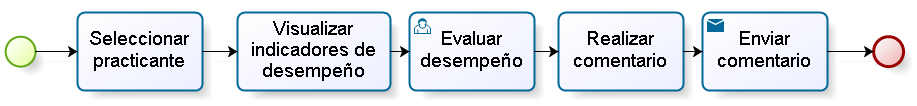
\includegraphics[scale=0.7]{./Figuras/Negocio/Registrar_comentarios}
				\end{center}
				\caption{Registrar comentarios}
				\label{fig:procesonegocioP_regComent}
		\end{figure}
		\item Recibir comentarios (Practicante): El Practicante puede visualizar los comentarios hechos por el Entrenador, para poder hacer las mejoras pertinentes y en la próxima rutina mejorar su desempeño.
	\end{itemize}
	
\end{enumerate}
\clearpage